\documentclass[a4paper, 12pt, twoside]{article}
%\usepackage[hungarian]{babel}
\usepackage{ae,aecompl}
\usepackage[T1]{fontenc}
\usepackage[utf8]{inputenc}
\usepackage{textcomp}
\usepackage{anysize}
% left right up down
\marginsize{3.2cm}{2.8cm}{2cm}{2cm}
\usepackage{setspace}
\setstretch{1.2}
\frenchspacing
%\pgfplotsset{compat=newest}
%\pagestyle{empty}
%\usepgfplotslibrary{ternary}
\usepackage{chemfig}
\usepackage{gensymb}
\usepackage{fancyhdr}
\usepackage{enumerate}
\usepackage{amsmath}
\usepackage{upgreek}
\usepackage{indentfirst}
\usepackage{sidecap}
\numberwithin{equation}{section}
\numberwithin{figure}{section}
\numberwithin{table}{section}
\hyphenation{hő-mér-sék-let-füg-gé-sét}
\usepackage{pgfplots}
\usepackage{pst-plot}
\usepackage{tikz}
\usepgfplotslibrary{colormaps}
\usetikzlibrary{pgfplots.colormaps}
%\usepgfplotslibrary{external}
%\tikzexternalize



\renewcommand\footrule{\begin{minipage}{1\textwidth}
%\hrule width \hsize height 2pt \kern 1mm \hrule width \hsize   
\hrule width \hsize height 1pt   
\end{minipage}\par}%

\renewcommand\headrule{
\begin{minipage}{1\textwidth}
%\hrule width \hsize \kern 1mm \hrule width \hsize height 2pt 
\hrule width \hsize height 1pt 
\end{minipage}}%

\pagestyle{fancy}
\fancyhf{}
%\fancyhead[LE,RO]{\leftmark}

%\setlength{\footskip}{40pt}

%\pagestyle{fancy}
%\fancyhf{}
%\usepackage{lastpage}
%\rfoot{Page \thepage \hspace{1pt} of \pageref{LastPage}}
%\lhead{\thesection}
%\cfoot{\itshape\textcolor{gray}{Fizikai Kémia gyakorlatok gyógyszerészeknek}}

\setcounter{tocdepth}{1}
%\thispagestyle{empty}
\title{Physical chemistry laboratory practice}

\author{\emph{written by:} \\ Barna Kovács \\ Sándor Kunsági-Máté \\ Géza Nagy \\ \\ \emph{translated by:} \\ András Kiss \\ \\ \\ \\ \\ \\ \\ \\

\includegraphics[width=0.2\textwidth]{fig/pte_logo.eps} \\
Department of General and Physical Chemistry \\ University of Pécs}

\begin{document}
\clearpage\maketitle
\thispagestyle{empty}
\newpage 
\tableofcontents
\newpage

\fancyhead[LE,RO]{Drug decomposition -- ,,GYB''}
\fancyhead[LO,RE]{\thesection}
\fancyfoot[LE,RO]{\thepage}
\fancyfoot[RE,LO]{\emph{Physical chemistry lab. practice for pharmacy students}}

%\setcounter{section}{7}
\section{Investigating the temperature dependence of drug decomposition}
\subsection{Introduction}

During this practice we study the pseudo first-order hydrolysis reaction of acetilsalicilic acid.
The rate constant of a first-order reaction can be written as:

\begin{equation}
\label{eq:divider}
        k
        =
        \frac
                {1}
                {t}
	\ln
	\frac{z}{z-x}
\end{equation}

where $t$ is time, $z$ is the initial concentration of the reagent, $x$ is the concentration of the product at time $t$.

The reaction rate depends on temperature, which is stated in the \emph{Arrhenius law}:

\begin{equation}
\label{eq:divider}
        \frac
                {d\ln k}
                {dT}
	=
	\frac
		{E}
		{\mathrm{R}T^2}
\end{equation}

after integration:

\begin{equation}
\label{eq:divider}
        k
        =
	A
	e^{-E/( \mathrm{R} T)}
\end{equation}

and

\begin{equation}
\label{eq:divider}
        \lg k
        =
        \lg A
	-\frac{E}{2.303 \mathrm{R}T}
\end{equation}

$A$ is the preexponential factor, $E$ is the activation energy, and R is the universal gas constant (R$ = 8.314$ J/Kmol). The factor 2.303 is the conversion form ln to lg.
Activation energy can be obtained graphically if we take the slope of the function $\lg k - 1/T$ and multiply it by 2.303 $\times$ 8.314. The dimension in this case for $E$ is J/mol.
If we measure $k$ on two different temperatures ($k_1$ and $k_2$ on $T_1$ and $T_2$ temperature), activation energy can be calculated as follows:

\begin{equation}
	E
	=
	2.303
	\times
	8.314
	\lg
	\frac{k_1}{k_2}
	\frac{T_1 T_2}{T_1-T_2}
\end{equation}

\subsection{Practice procedures}

Alkaline hydrolysis of acetylsalicylic acid (Fig. \ref{fig:salicilsav}) is a pseudo first-order reaction. 
\begin{figure}
\centering
\schemedebug{false}
\schemestart
	\footnotesize \chemname{\chemfig{*6(-=-(-O-[::-60]([::-60]=O)-)=(-(-[::-60]OH)=[::60]O)-=)}}{acetylsalicylic acid}
	\footnotesize \+
	\footnotesize \chemfig{OH^{-}}\arrow(.mid east--.mid west){->[k][]}
	\footnotesize \chemname{\chemfig{*6(-=-(-OH)=(-([::-60]-OH)=[::60]O)-=)}}{salicylic acid} + CH$_3$COO$^-$
\schemestop
\caption{Alkaline hydrolysis of acetylsalicylic acid.}
\label{fig:salicilsav}
\end{figure}
The reaction is quite slow on room temperature, therefore we conduct our measurements at a higher temperature.
To determine the rate constant $k$, we need to know the change in concentration of the reactants or the products as a function of time.
In this practice, we will use spectrophotometry after forming an Fe$^{3+}$ salicilate complex by adding FeCl$_3$ to the samples. The complex has a deep violet color, and its absorbance is directly proportional to the concentration of the complex, therefore to the concentration of the product salicilate as stated by \emph{Lambert-Beer's law}:

\begin{equation}
\label{eq:beer}
        A
        =
	\epsilon
	l
	c
\end{equation}

where A is absorbance, $\epsilon$ is the molar decadic absorption coefficient, $l$ is the length of the solution block the light is passing through, and $c$ is the concentration.
We take known volumes of samples from the alkaline reaction vessel, and suddenly decrease [OH$^-$] and temperature by adding NaOH and putting the samples on ice.
If the measured absorbance is above 2 A.U., dilution is necessary, since over this value the relationship between $c$ and $A$ is not linear anymore. To determine the product concentration at $t = \infty$ (which equals to the reactant concentration at $t = 0$), we take samples at the and of the practice. We carry out the measurements at two different temperatures, determined by the instructor (usually 313 and 353 K).

Pulverize an \emph{Aspirin} tablet in a mortar with the help of a pestle, dissolve it a small amount of deionized water, then filter it into a 100 cm$^3$ measuring flask, and fill it up to 100 cm$^3$. This will be the stock solution. The stock solution obtained in this way will be most likely saturated\footnote{An \emph{Aspirin} tablet has 500 mg acetylsalicylic acid in it, and its solubility in water is 2 - 4 g / L, depending on temperature.}

\textbf{Starting and following the reaction:}

\begin{enumerate}[(a)]
\item Determining the initial concentration $z$ of acetylsalicylic acid. Pipette 2-2 cm$^3$ sample from the stock solution into two Erlenmeyer flasks with bottlecaps (low and high temp.), and add 3-3 cm$^3$ 0.25 M NaOH solution to them. Put them into the two thermostats after labeling them. At the end of the practice we stop the reaction. It should be complete, but we should treat these solutions as the others to rule out any artifacts. ,,Stop the reactions'' by adding 2-2 cm$^3$ 0.25 M HCl solution and 3-3 cm$^3$ FeCl$_3$, then fill the flasks up to 100 cm$^3$ with deionized water.

\item Determining concentration $x$ at time $t$. Put one half of the remaining stock solution into an Erlenmeyer and the other half into another Erlenmeyer flask. Close the flasks, label them, and put them into their respective thermostats. Add 5 cm$^3$ buffer solution (ask the technician), and start a stopwatch. By adding the buffer solution the reaction starts ($t$ = 0). Without taking out the flask, take 2 cm$^3$ samples from them at 15, 20, 25, 30 and 35 minutes after the reaction has started, and put them into separate, labeled 25 cm$^3$ measuring flasks you prepared beforehand. Prepare them by adding 0.5 cm$^3$ 0.25 M HCl solution (this will stop the \emph{alkaline hdydrolysis}), and 0.5 cm$^3$ 0.1 M FeCl$_3$ solution (to form the complex and make the product visible for spectrophotometry). Fill the remaining volume in the 25 cm$^3$ flasks with deionized water. Start the two reactions by shifting one by $1 - 2$ minutes, so you don't have to take samples at the same time from the two reactions.
\end{enumerate}

\textbf{Measuring absorbance and calculating concentration}. Both the initial and the instantaneous concentration at time $t$ will be measured spectrophotomertically. Find the users manual next to the instrument, or ask the instructor to help. To calculate the concentration from absorbance use the factor $b = 8.3~(mol/dm^3) / AU$. This is the concentration of the theoretical solution, whose absorbance is 1 AU, if $d = 1~cm$, where $d$ is the length of solution block in the path from source to detector.

\subsection{Results to submit}

\begin{enumerate}
\item Measured and calculated data in table (use table \ref{table:tablazatos} as reference).
\item Calculate the rate constants (table \ref{table:seb}.) for both temperatures, and calculate standard deviation\footnote{Standard deviáció, $s=\sqrt{\frac{\Sigma(x_i-\overline{x})^2}{n-1}}$}.
\item From the temperature dependence of the rate constant, calculate the rate constant for 20 $\celsius$-on (293 K) graphically by plotting $\lg k$ as a function of $1/T$.
\item Calculate $E$ and $A$ by substituting into the integrated form of the Arrhenius equation:
	\begin{enumerate}
		\item E [kJ mol$^{-1}$]
		\item $\lg$ A [$s^{-1}$]
		\item A [s$^{-1}$]
	\end{enumerate}
\end{enumerate}

\begin{table}[h!]
\caption{Measured and calculated data.}
\centering
T = ... K, $z$ = ... mg/100 cm$^3$
\begin{tabular}{|c|c|c|c|c|c|}
\hline
reaction time, s&dilution&A&x, mg / 100 cm$^3$ &(z-x), mg / 100 cm$^3$ & $k$, s$^{-1}$ \\
\hline
... & ... & ... & ... & ... & ... \\
\end{tabular}
\label{table:tablazatos}
\end{table}

\begin{table}[h!]
\caption{Temperature dependence of the rate constant.}
\centering
\begin{tabular}{|c|c|c|c|c|}
\hline
T, K& 1/T & $\overline{k}$ (average), s$^{-1}$ & $\lg k$ & standard deviation \\
\hline
... & ... & ... & ... & ... \\
\end{tabular}
\label{table:seb}
\end{table}

\vfill

%Updated and translated by András Kiss in 2016.

\newpage
\clearpage
\fancyhead[LE,RO]{Ionselective electrodes -- ,,SZEL''}
\fancyhead[LO,RE]{\thesection}
\fancyfoot[LE,RO]{\thepage}
\fancyfoot[RE,LO]{\emph{Physical chemistry lab. practice for pharmacy students}}

%\setcounter{section}{7}
\section{Determination of selectivity coefficient of ion-selective electrode}
\subsection{Introduction}

Ion-selective electrodes are potentiometric sensors, that allow the selective determination of the activity of certain ions.
They are widely used in the clinical diagnostics for routine measurements: automatic blood analisators measure the Na$^+$ and K$^+$-ion activity in blood samples. One more example is the determination of F$^-$-ion in tap water, even if there are interfering ions such as Cl$^-$ or OH$^-$. Their function is based on a selective membrane, which can be ionophore based (Na$^+$ and K$^+$), or lattice vacancy based (F$^-$). An example for the latter is the F$^-$ ion-selective electrode, which is based on a europium doped lanthanum fluoride crystal.

The equation that describes the behaviour of these electrodes is the Nernst-equation:

\begin{equation}
\label{eq:nernst}
	E
	=
	E^0
	+\frac{RT}{z_i F}
	ln(a_i)
\end{equation}

where $z_i$ is the signed valence of the primary ion (the ion that the electrode is selective to), $a_i$ is its activity.
According to the equation, for cation elective electrodes the electrode potential ($E$) is increasing with increasing actvity, and for anion selective ones, it decreases.
Because of deviations from the theoretical behaviour, in practice, we use the following, experimental equation:

\begin{equation}
\label{eq:exp}
	E
	=
	E^0
	\pm S ln(a_i)
\end{equation}

where $S$ is the slope of the linear part of the electrode calibration curve, which can be measured.
In real, multi-component samples, the potential of the ion-selective electrodes is influenced by the so-called \emph{interfering ions}, but in fact, more or less by every ion in the sample to some (small) extent.
For this reason, using eqs. \ref{eq:nernst} and \ref{eq:exp} will introduce error during evaluation.
To take into account these deviations we use the concept of \emph{selectivity coefficient} ($k_{pot}$). With this we can rewrite the equations as such: 

\begin{equation}
\label{eq:nikolsky}
E=E^0 + \frac{RT}{z_iF} \ln \left [ a_i + \sum_{j} \left ( k_{ij}a_j^{z_i/z_j} \right ) \right ]
\end{equation}

This is the Nikolsky equation. $a_j$ is the activity of the $j$th interfering ion, $z_j$ is its charge, $k_{pot}$ $i, j$ is the selectivity coefficient of the $j$th ion.
The selectivity coefficient shows how much more sensitive is the electrode towards the primary ion, then towards to the interfering ion.
For instance, if $k = 10^{-2}$, the activity of the $j$ ion must be hundredfold of the $i$ primary ion to have the same effect on the electrode potential (increase or decrease it to the same extent).
There are two main methods for determining the selectivity coefficient: the mixed and the separate solution methods.

In the mixed solution method, ion activity of the $j$ interfering ion is constant, and we increase the activity $i$ primary ion, and measure the potential response.
After plotting the data fig. \ref{fig:Q}, we find $Q$. Then, we calculate the selectivity coefficient as follows:

\begin{equation}
\label{eq:szel1}
	k_{i,j}^{pot}
	=
	\frac{(a_i^{z_j})_Q}{a_j^{z_i}}
\end{equation}


\begin{figure}
\centering
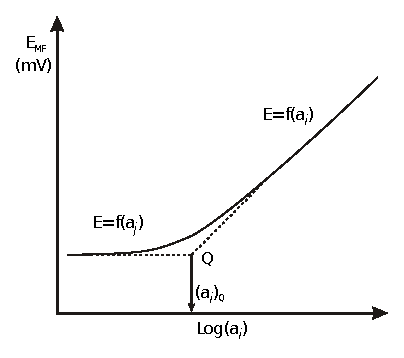
\includegraphics{ion1.eps}
\caption{Using the mixed solution method to determine the selectivity coefficient.}
\label{fig:Q}
\end{figure}

When using the separate solution method, we need to record two calibration curves.
First, at zero interfering ion activity, we make a calibration of primary ion $i$, then at zero primary ion $i$ activity, we make a calibration plot of interfering ion $j$.
After obtaining these two curves, the selectivity coefficient can be obtained as seen in fig. \ref{fig:ion2}, taking either

\begin{enumerate}[(a)]
\item activities corresponding to the same potentials:

\begin{equation}
\label{eq:azonospot}
        k_{i,j}^{pot}
        =
        \frac{a_i}{a_j^{z_i/z_j}}
\end{equation}

\item or potentials corresponding to the same activities:

\begin{equation}
\label{eq:azonosakt}
        \lg k_{i,j}^{pot}
        =
        \frac{(E_2-E_1)zF}{2.303RT}
	=
	\frac{\Delta E}{S}
\end{equation}

\end{enumerate}

There are a number of factors that influence the selectivity coefficient: ionic strength, method, etc...
As it can be seen, from relationships \ref{eq:azonospot} and \ref{eq:azonosakt}, the drawback of the separate solution method is that it assumes, that the valence of the primary and interfering ion is equal, and that the sensitivity towards them is the same.
For this reason, selectivity coefficients obtained with this method are regarded as approximations, and the much better mixed solution method is preferred.

\begin{figure}
\centering
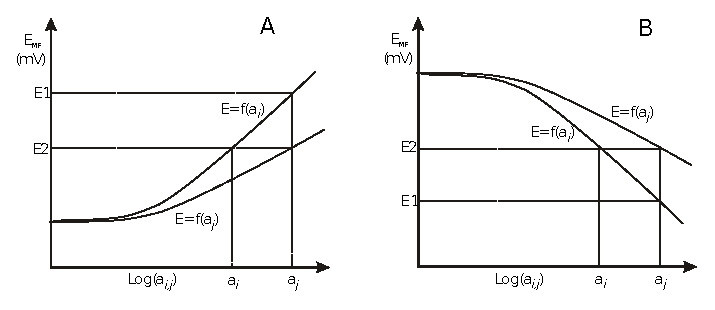
\includegraphics{ion2.eps}
\caption{Determining the selectivity coefficient with the separate solution method for positive (A) and negative (B) ions.}
\label{fig:ion2}
\end{figure}

\subsection{Practice procedures}
The purpose of this practice is to study the function of potassium or fluoride ion-selective electrodes (ask the instructor which one).
Your first task is to prepare a dilution series of soluions of the primary ion. Use salts KCl or NaF.
Prepare 100 ml 10$^{-2}$ mol$\cdot$dm$^{-3}$ solution using a salt of the primary ion. 
Then make a tenfold dilution by taking out 10 ml from this solution, and putting it in another, clean 100 ml measuring flask. Fill it up to 100 ml with deionized water. Continue making dilution by always using the previous solutions, until you reach a concentration of 10$^{-6}$ mol$\cdot$dm$^{-3}$. 
Pour a small amount of each into separate, labeled beakers, so that the electrodes can submerse into them with their active area.
Then start with the most dilute solution by putting the measuring and the reference electrodes into it. Wait 1 minute, and write down the potential.
Move on to the next solution (10$\times$ more conc.), wait another 1 minute, and record the data.
Carry out measurements in all five solutions advancing from dilute to concentrated, repeat it altogether 3 times. Carefully rinse the electrodes between series.

\subsubsection{Determining the selectivity coefficient using the separate solution method}
Repeat the previous procedure, but use a salt of the interfering ion to prepare the first solution, the do the dilutions. It's important to use deionized water free of potassium, sodium, chloride and fluoride ions as much as possible. Ask the technician for ultrapure water. 

\subsubsection{Determining the selectivity coefficient using the mixed solution method}
For this method prepare another dilution series by using a salt of the primary ion, but instead of deionized water, use a 10$^{-2}$ M solution of the interfering ion as solvent. In this way, the interfering ion concentration will be constant in all of the solutions, but the primary ion concentration will vary just like in the first experiment.

\subsection{Evaluation}
\begin{enumerate}
\item Find the activity coefficients for the primary and interfering ions online, and calculate the activities from the concentrations.

\item Plot the $\lg a_i$ -- $E$ functions as seen in the diagrams above. 

\item Determine the slope of the linear part by linear fitting for each graph.

\item Determine the lower limit of detection of the electrode towards the primary ion ($Q$ when there is no interfering ion).

\item Calculate the selectivity coefficients using all 3 methods (1 mixed solution method and 2 separate solution methods).

\item For the separate solution method, plot the two curves in the same diagram.
\end{enumerate}

\subsection{Results to submit}
Lower limit of detecction towards the primary ion, 2 selectivity coefficients from the separate solution method, and 1 from the mixed solution method.
Five calibration diagrams, each with linear fits on the linear section.

\vfill
%\center
%Updated and translated by András Kiss assistant lecturer 2016.

\newpage
\fancyhead[LE,RO]{Determination of pK with conductometry -- ,,PKVEZ''}
\fancyhead[LO,RE]{\thesection}
\fancyfoot[LE,RO]{\thepage}
\fancyfoot[RE,LO]{\emph{Physical chemistry laboratory practice}}

%\setcounter{section}{1}
\section{Determination of dissociation constants of weak acids with conductometry}
\subsection{Introduction}
According to Ohm's law, the current passing through between two points and the potential difference between those two points are in linear relationship:

\begin{equation}
\label{eq:ohm}
	U
	=
	I
	\cdot
	R
\end{equation}

where $R$ is the factor of proportionality, called \textbf{electrical resistance}. Its dimension is ohm ($\ohm$).

Specific resistance is the longitudinal resistance of a conductor which is 1 m long and has a cross section of 1 m$^2$ (1 mm$^2$ in practice). 

In electrochemistry it is often more simple to use the reciprocal of these quantities. The reciprocal of resistance is conductivity, its dimension is Siemens, S = 1/$\ohm$. The reciprocal of specific resistance is specific conductivity. The specific conductivity of an electrolyte is the conductivity we measure if the two electrodes have a surface area of 1 cm$^2$, they are 1 cm apart, they are made of an inert metal (gold, platinum), and they are submersed in the electrolyte. Its dimension is S $\cdot$ cm$^{-1}$. It depends on concentration, temperature, and it's a unique property of every material.

Molar specific conductivity ($\Lambda _m$) is the ratio of the specific conductivity and the concentration:

\begin{equation}
\label{eq:lambdam}
        \Lambda_m
        =
        \frac
		{\kappa 1000 }
		{c}
	=
	\kappa V
\end{equation}

where $c$ is concentration (mol$\cdot$dm$^{-3}$), and $V$ is dilution.

Kohlrausch found that the limiting molar conductivity (molar conductivity of an infinitely dilute solution) of anions and cations are additive: the conductivity of a solution of a strong electrolyte is equal to the sum of conductivity contributions from the cation and anion:

\begin{equation}
\label{eq:kohlrausch2}
	\Lambda _m^0
	=
	\lambda _a^0 \nu _a z_a + \lambda _k^0 \nu _k z_k
%	/1000
\end{equation}

where $z_a, z_k$ are the valence of the ions, $\nu _a, \nu _k$ are stochiometric factors, $\lambda _a^0$ and $\lambda _k^0$ are the limiting molar conductivities for the anions and the cations.

The conductivity of weak electrolytes can be described as follows:

\begin{equation}
\label{eq:lambdam}
        \lambda_c
        =
        \alpha
	\lambda_0
\end{equation}

where $\alpha$ is the degree of dissociation, $\lambda _0$ is the limiting molar conductivity.
The dissociation constant $K_d$ of a weak acid can be calculated from its concentration and its degree of dissociation:

\begin{equation}
\label{eq:kd}
        K_d
        =
        \frac{\alpha^2 c}{1-\alpha}
\end{equation}

It is worth noting however, that $K_d$ -- based on the Debye-Hückel theory -- depends on the permittivity of the media and temperature.

If we express $\alpha$ from \ref{eq:lambdam}, we get \emph{Ostwald's law of dilution}:

\begin{equation}
\label{eq:ostwald}
        K_d
        =
        \frac{\lambda_c^2 c}{\lambda_0^2 - \lambda_0\lambda_c}
\end{equation}

That means we can determine $K_d$ from conductometric measurements. $\lambda_c$ can be measured directly, while $\lambda_0$ can be obtained with the following method. By rearranging eq. \ref{eq:ostwald} we get

\begin{equation}
\label{eq:ostwald2}
        \frac{1}{\lambda_c}
        =
	\lambda_c
	c
	\frac{1}{K_d \lambda_0^2}
	+\frac{1}{\lambda_0}
\end{equation}

If we plot $1/\lambda_c$ as a function of $\lambda_c c$ (which is nothing but $\kappa$), we get a straight line whose y interception is $1/\lambda_0$. And knowing $\lambda_c$ and $\lambda_0$ we can calculate $K_d$.

Additionally, we have to consider these:

\begin{enumerate}[(a)]
\item The solvent also contributes to the conductivity of the solution. Therefore we substract the conductivity of the pure solvent ($G_{\text{solvent}}$) from each measurement carried out in the solutions of that solvent.

\item In practice, we don't use the conductivity cell from the definition of specific conductivity. Instead, the more practical ,,bell electrodes'' are used. To obtain specific conductivity from the conductivity values measured with these cells, we multiply every value with the cell constant $C$ (dimension:  m$^{-1}$ or cm$^{-1}$).

The cell constant shows the relationship between solution with a known specific conductivity ($\kappa_{ref}$) and the conductivity measured with cell used in practice ($G_{\text{measured}}$):

\begin{equation}
\label{eq:c}
	C
	=
	\kappa_{\text{ref}}/G_{\text{measured}}
\end{equation}

\end{enumerate}

Based on this, we can calculate the contribution of solute to the conductivity of the solution: $\kappa_{\text{korr}} = (G_{\text{solution}} - G_{\text{solvent}})C$, where $\kappa_{\text{korr}}$ is the specific conductivity of the solution taking into account that of the solvent and the cell constant.

Therefore, specific molar conductivity of a weak acid is:

\begin{equation}
\label{eq:c}
        \lambda
        =
        \kappa_{korr}
	V
\end{equation}


\begin{figure}[h!]
\centering
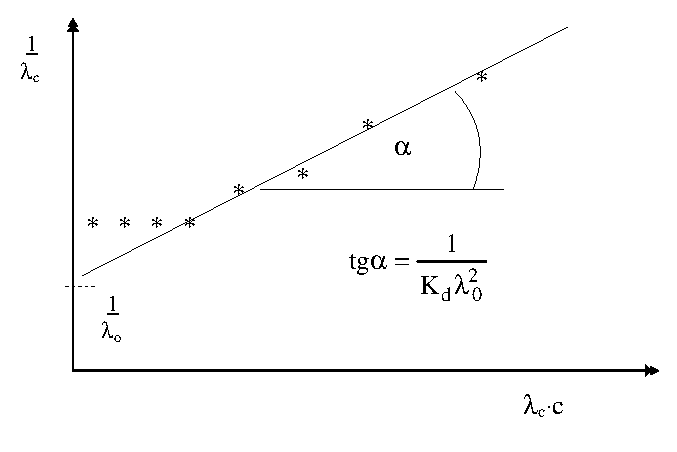
\includegraphics{fig/lambda0.eps}
\caption{Obtaining the limiting molar conductivity ($\lambda_0$).}
\label{fig:}
\end{figure}

\subsection{Practice procedures}

Rinse the electrode of the conductometer several times (4 - 5) with deionized water, the with ultrapure water ($\kappa$ < 1 $\upmu$S/cm). Ask the technician for ultrapure deionized water.

Prepare 20 v/v\% solution from an alcohol selected by the instructor. Then prepare two weak acid solutions (the weak acid is also selected by the instructor), from the stock solution (1 mol$\cdot$dm$^{-3}$) by pipetting 2.00 cm$^3$ into two 100 cm$^3$ measuring flasks, and then filling one with the 20 v/v\% alcohol solution, the other with ultrapure deionized water up to 100 cm$^3$.

Carry out the conductivity measurements in a measuring cilinder. Pour the water based solution into the cilinder and measure its conductivity. Then, pipette 25 cm$^3$ from the cilinder into a clean 50 cm$^3$ measuring flask, fill it up with ultrapure deionized water (2$\times$ dilution), and measure the conductivity of the new solution after carefully rinsing it with ultrapure deionized water. Repeat the dilution and measurement 3 times. Then do the same with the alcohol based solution, but using the 20 v/v\% alcohol solution for the dilutions and rinsing.

Note and record the temperature measured by the built-in thermometer of the electrode for each measurement.

Finally, measure the conductivity of the solvents as well (for the correction).
Then, to obtain the cell constant, measure the conductivity of 0.01 M KCl solution, and write down the temperature as well. Based on table 

Figure \ref{fig:vez} shows the schematics of a conductometric cell. A well-defined, inert electrode pair is submersed into an electrolyte, and the voltage drop between them is measured. Alternating current is used to avoid polarization and electrolysis.

\begin{figure}
\centering
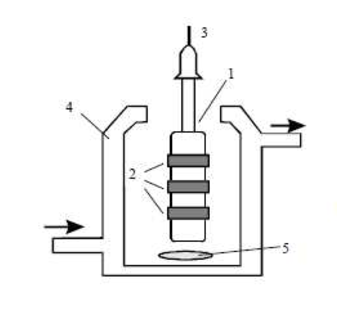
\includegraphics{fig/cond.eps}
\caption{Schematics of a conductometric cell. 1 - ,,bell electrode'', 2 - platinized platinum rings, 3 - electrical connection, 4 - double walled vessel, 5 - magnetic stirrer.}
\label{fig:vez}
\end{figure}

\subsection{Evaluation}

\begin{enumerate}
\item Calculate the cell constant.
Present the recorded data in such a table:

\begin{table}[!h]
\centering
\begin{tabular}{|c|c|c|c|c|c|c|c|}
\hline
c (mol $\cdot$ dm$^{-3}$) & G$_{\text{measured}}$ & $\kappa_{\text{korr}}$ (S $\cdot$ cm$^{-1}$) & $\lambda_c$ & $1/\lambda_c$ & $\lambda_c c$ & $\alpha$ & $K_d$ \\
\hline
... & ... & ... & ... & ... & ... & ... & ... \\
\end{tabular}
\label{table:vez}
\end{table}

\item Determine $\lambda_0$ graphically. Knowing $\lambda_c$ and $\lambda_0$, calculate $\alpha$ and $K_d$ for each concentration.

\end{enumerate}



\newpage
\fancyhead[LE,RO]{Catalytic oxidation -- ,,AO''}
\fancyhead[LO,RE]{\thesection}
\fancyfoot[LE,RO]{\thepage}
\fancyfoot[RE,LO]{\emph{Physical chemistry lab. practice for pharmacy students}}

%\setcounter{section}{7}
\section{Electrochemical study of the catalytic oxidation of vitamin C}
\subsection{Introduction}
In this practice we will use an electrochemical method, voltammetry to study the catalytic oxidation of vitamin C. It is an essential vitamin for humans. Its spontanaeous oxidation is well known:

\begin{equation}
\label{eq:divider}
        C_6 H_8 O_6
	+
	1/2 O_2
        =
	C_6 H_6 O_6
	+ H_2O
\end{equation}

The reaction is catalyzed by multivalent metal ions. If there is excess oxygen, the reaction becomes pseudo first-order. In this case, the measured rate constant is an \emph{apparent rate constant}. Let's look at a simple reaction:

\begin{equation}
\label{eq:divider}
        A
        +
        B
        =
        P
\end{equation}

In this reaction, product $P$ is formed from reactants $A$ and $B$. The rate equation is

\begin{equation}
\label{eq:rate_differential}
	v
	=
	\frac{d[A]}{dt}
	=
	-\frac{d[P]}{dt}
	=
	k[A]
\end{equation}

To determine $k$, we can either measure the change in $[A]$, $[B]$ or $[P]$ as a function of time $t$. Consider the change in $[A]$. Assume, that the initial ($t = 0$) concentration is $[A_0]$. Then we can solve the differential equation \ref{eq:rate_differential} by integrating:

\begin{equation}
\label{eq:rate}
        \int_{[A_0]}^{[A]}
        \frac{d[A]}{dt}
        =
        -k \int_0^t
	dt
\end{equation}
 
The solution is:

\begin{equation}
\label{eq:rate}
        ln
	\frac{[A]}{[A_0]}
        =
        -kt
\end{equation}

and

\begin{equation}
\label{eq:rateln}
        [A]
	=
	[A_0]
	e^{-kt}
\end{equation}

In a first-order reaction, concentration changes exponentially in time, and the logarithm of concentration changes linearly as a function of time. By using eq. \ref{eq:rateln}, we can decide if a reaction is first-order or not. This can be done by plotting ln$[A]$ as a function of time, and see if the points fit on a line or not. If they do, it's a first-order reaction, and the slope is the rate constant $k$.

\subsection{Practice procedures}
We will use voltammetry to determine the concentration of ascorbic acid at any time $t$. First, make a calibration plot:

\begin{enumerate}
\item Start by preparing 50 ml 10 mM stock solution, dissolved in deionized water.

\item Then take a clean 20 - 50 ml beaker, and measure 10 ml of 0.1 M NaCl solution into it. Place the beaker on a magnetic stirrer, and put a magnet into the beaker. Put the electrodes into the solution. We will use carbon paste working electrode, Ag/AgCl reference electrode, and a platinum auxiliary electrode.

\item Record a cyclic voltammogramm from 0 to 0.8 V, with a scanrate of 100 mV/s. Adjust the current range if necessary.

\item Then start increasing the ascorbic acid concentration (now it's zero), by adding small volumes (30 $\upmu$l) from the stock solution. Record a CV after every addition. Repeat it 10 times, so you have 11 measurements. Now you have data for the calibration curve. Calculate the concentrations at home. (For example if you add 100 $\upmu$l, $c = n/V = (0.1~mol\cdot L^{-1} \times 0.0001~L) / 0.0101~L = 9.9\cdot10^{-3}~mol\cdot L^{-1}$.) Prepare a table to record the data in. (First column: added total volume of ascorbic acid, second column: anodic peak current, $i_{pa}$.)
\end{enumerate}

Then, we will follow the catalytic oxidation of ascorbic acid by measuring its concentration with voltammetry:

\begin{enumerate}
\item To study the catalytic oxidation of ascorbic acid, we will use a double walled, thermostatted reaction vessel. Start the thermostat. Put 80 ml of 0.1 M NaCl solution into it. Add 100 $\upmu$l of 0.1 M CuCl$_2$. This will serve as a catalyst.
\item Start the oxygen pump. This serves two purposes. First, it supplies the reaction with plenty of oxygen, so it becomes pseudo first-order. Additionally, it stirs the solution.
\item Take a small sample out, and record a CV the same way you did in the calibration measurements. The volume doesn't matter, but it should be enough for the electrodes to have their acitve area submersed. Put the sample back into the reaction vessel after the measurement is complete.
\item Add 1 ml of stock solution to the reaction vessel. Start a stopwatch at the moment of addition. This is when the reaction starts.
\item At $t = 5, 10, 15, 20, 25, 30, 35, 40$ minutes, take samples and record a CV in them. Always put the sample back into the reaction vessel.
\end{enumerate}

\subsection{Results to submit}

\begin{enumerate}
\item Cyclic voltammogramms of the calibration measurements.
\item Cyclic voltammogramms of the measurements for the catalytic breakdown.
\item Calibration plot ($c - i_{pa}$). $i_{pa}$ is the anodic peak on the CV. Its magnitude is proportional to the concentration of ascorbic acid. This relationship is what we will use in the determination of the concentration. From the calibration plot, the concentration of ascorbic acid in an unknown solution can be determined from the anodic peak.
\item $t - c$ table for the catalytic breakdown. First column: time, second column: concentration of ascorbic acid calculated from the anodic peak currents, using on the calibration plot.
\item $lnc - t$ plot. This is the plot on which you should fit a linear equation. Its slope will be the \textbf{rate constant}. This is the end result of the practice. Write a conlcusion: ,,Rate constant of the catalytic breakdown of ascorbic acid, based on my measurements in these conditions (list conditions here) is $k = ... s^{-1}$.
\end{enumerate}

\newpage
\fancyhead[LE,RO]{Sucrose inversion -- ,,ELS''}
\fancyhead[LO,RE]{\thesection}
\fancyfoot[LE,RO]{\thepage}
\fancyfoot[RE,LO]{\emph{Physical chemistry lab. practice for pharmacy students}}

%\setcounter{section}{7}
\section{Investigation of sucrose inversion with polarimetry}
\subsection{Introduction}
The purpose of the studies in reaction kinetics is to reveal the underlying mechanisms, for which the knowledge of the order or partial order regarding the reactants is really helpful.
The general rate equation for homogeneous reactions is:

\begin{equation}
\label{eq:general}
	r
	=
	k[A]^{\beta_a}[B]^{\beta_b}...[N]^{\beta_n}
\end{equation}

where $\beta_a$, $\beta_b$ and $\beta_n$ are the partial order of the respective reactants, and $\beta = \beta_a + \beta_b + ... + \beta_n$ is the overall order of the reaction.

If there is concentration -- time data available and we know the order of the reaction, the rate constant can be calculated.

\paragraph{Using the rate equations.}
It is possible to use the indefinite integral form of first order reactions for graphical evaluations:

\begin{equation}
\label{eq:2}
	\ln 
	\frac{[A]}{[A]_0}
	=
	- k
	t
\end{equation}

Plotting $\ln [A]$ as a function of time we get a staright line, whose slope is $-k$, the rate constant (fig. \ref{fig:els_1}). Note that the slope of the $\ln ([A]/[A]_0) - t$ and $\ln [A] - t$ functions are the same, since $\ln ([A]/[A]_0) = \ln [A] - \ln [A]_0$ and $\ln [A]_0$ is constant.

\begin{figure}[b]
\centering
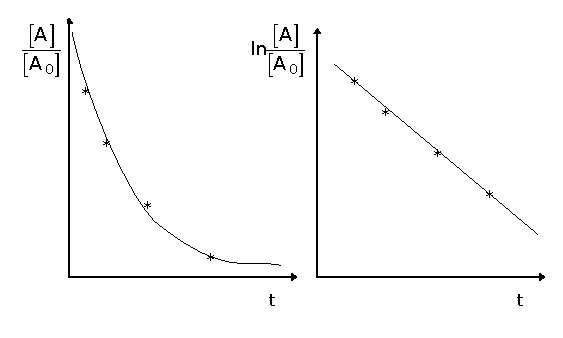
\includegraphics{fig/els1.eps}
\caption{Determining the rate constant of a first order reaction.}
\label{fig:els_1}
\end{figure}

Usually concentration is not measured directly, but a quantitiy that is proportional to concentration is measured. We will denote this quantitiy as $z$ in general.
It is easy to see that the difference between $z_0$ at time $t = 0$ and $z_\infty$ at time $t = \infty$ is proportional to $[A]_0$ and the product concentration at the end of the reaction ($t = \infty$), if there is a linear relationship between $z$ and $[A]$.
Then, it is possible to express the concentration $[A]$ at any time $t$ if the measured signal $z_t$ at time $t$ and $z_{\infty}$ is known.
Substituting to eq. \ref{eq:2}, we get

\begin{equation}
\label{eq:3}
        \ln 
        \frac{z_{\infty}-z_t}{z_{\infty}-z_0}
        =
        - k
        t
\end{equation}


\paragraph{Guggenheim's method.}
To use eq. \ref{eq:3}, to determine the rate constant of a first order reaction, the knowledge of the physical parameter $z$ at both $t=0$ and $t=\infty$ is necessary.
When the reaction is too fast or too slow however, measuring $z_0$ or $z_\infty$ might prove to be problematic due to technical difficulties.
To circumvent these difficulties one could use \emph{Guggenheim's method}. To do this, measure $z_t$ at $t_1, t_2, t_3, ... , t_n$ and at $t_1+\Delta t, t_2+\Delta t, t_3+\Delta t, ... , t_n+\Delta t$, where $\Delta t$ is a constant time interval.
For instance if we measured $z$ at $t= 12, 18$ and $27$ seconds, and $\Delta t = 30 s$, we measure $z$ at 42, 48 and 57 seconds as well.

\begin{figure}[h]
\centering
\label{fig_els2}
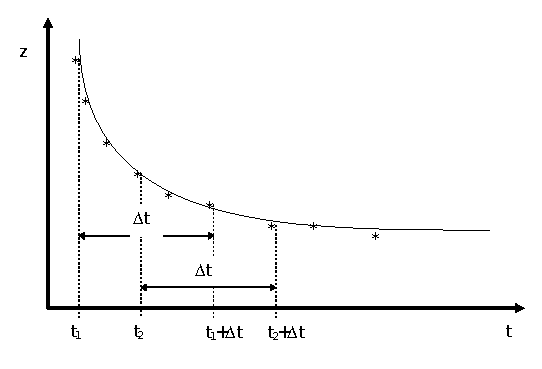
\includegraphics{fig/els2.eps}
\caption{Determining the rate constant of a first order reaction using \emph{Guggenheim's method}.}
\end{figure}

First we substitute $t$ and $t + \Delta t$ into the exponential form of eq. \ref{eq:3}, then rearrange the resulting equation:

\begin{equation}
\label{eq:4}
	z_t - z_{\infty}
	=
	(z_0 - z_{\infty}) e^{-kt}
\end{equation}

\begin{equation}
\label{eq:5}
	z_{t + \Delta t} - z_{\infty} = (z_0 - z_{\infty}) e^{-k(t+\Delta t)}
\end{equation}

Then substract eq. \ref{eq:5} from \ref{eq:4} to get

\begin{equation}
\label{eq:6}
        \ln (z_t - z_{t+\Delta t})
	=
	-kt
	+ \ln (z_0 - z_{\infty}) (1- e^{-k \Delta t})
\end{equation}

The second term on the right side is constant, since $z_0$ and $z_\infty$ does not change during the reaction (we don't add or remove reactants or products), and $\Delta t - t$ was chosen to be constant.
Thus, if we plot the left side as a function of $t$, we get a linear equation, whose slope is $k$, the rate constant.
Notice that for this method to work, we don't need to know either $z_0$ nor $z_\infty$. 
It must be mentioned however that one should choose $\Delta t$ carefully, preferably it should be as big as possible.
The estimation will be more precise if we measure in a small range of conversion, and $\Delta t$ approaches the half life ($t_{1/2}$) of the reaction.

\paragraph{Method of initial rates.}
Usually it's not possible to follow the concentration changes of all components in a reaction, nevertheless, the reaction order and rate constant is possible to measure anyway. Let's take a logarithm of both sides of eq. \ref{eq:general}: 

\begin{equation}
\label{eq:log}
	\ln r
	=
	\ln k
	+ \beta _a \ln [A]
	+ \beta _b \ln [B]
	+ ...
	+ \beta _n \ln [N]
\end{equation}

If we keep the concentration of every component constant except for example $A$, and we measure the rate constant at several different $[A]_0$, the we get a linear equation when we plot $\ln r$ as a function of $\ln [A]_0$. The slope of this equation is $\beta _a$, the partial order with respect to $A$.
This is true only at low conversion range, ie. the initial part of the reaction. The measurements must be done at time instances when $t << 0.05 t_{1/2}$.

\subsection{Investigating the inversion reaction of sucrose}
Sucrose is a disaccharide, which undergoes hydrolysis in acidic medium. As a result, D-glucose and D-fructode are being produced:

\begin{equation}
\label{eq:inversion}
	C_{12}H_{22}O_{11} + H_2O = C_6H_{12}O_6 + C_6H_{12}O_6
\end{equation}

If the solution is dilute enough, this becomes a pseudo first order reaction, because the ,,concentration of water'' does not change significantly.
The reaction occures in neutral solutions as well, but very slowly. Dilute acids will catalyse the reaction, and the reaction rate will be proportional with the concentration of the acid.
Since the reaction can be regarded as first order reaction, with eq. \ref{eq:3} the rate constant can be calculated if we measure a physical parameter that is proportional with the concentration of any of the components in the reaction.
In this practice we will use rotation of light that is passing through the solution.
In our system there are several optically active components: the solution of sucrose rotates light to the right ($+$), the products rotate light to the left ($-$).
This phenomenon is a result of the chirality of chemical compounds.
The speed of light in the optically active media is different for light polarized to the right and left.
Thus, there is a shift in phase when light hits the detector. If we use \emph{polarized} light, there is only light with a certain rotational angle, and it's possible to measure the phase shift.

In a cuvette with a length $l$, rotation is defined by

\begin{equation}
\label{fig:rotation}
	\alpha
	=\frac{10 \pi l}{\lambda}
	(n_l -  n_d)
\end{equation}

where $\lambda$ is the wavelength of light in cm, $n_l$ is the refractive index of light polarized to the left, $n_d$ is that of light polarized to the right.
Specific rotation is the rotation angle which is observed in a solution with a concentration of 1 g/cm$^3$ when $l = 1$ dm.
Since rotation depends on waveength and temperature, usually it is referenced to the \emph{D line} of sodium for either 20 or 25 $\celsius$.


\subsection{Practice procedures}
Prepare 100 cm$^3$ 30 m/m\% sucrose solution and 50 cm$^3$ 5 M HCl. To have a complete reaction at the end of the practice, first assemble the following reaction: 10 cm$^3$ sucrose solution $+$ 10 cm$^3$ HCl. Put it in a 50 $\celsius$ thermostat. By the end of the practice, the reaction should have been undergone completely. Leave it there for now, and continue with the $t = 0$ solution. Do this by creating a solution of 10 cm$^3$ sucrose solution $+$ 10 cm$^3$ H$_2$O. In this solution the reactions proceeds quite slowly, and it will not change significantly during the practice. This is the initial state, since there is only sucrose in the solution, and no glucose or fructose. You can take your time and familiarize yourself with the polarimeter.

Turn on the \emph{Krüss P1000-LED} polarimeter. This instrument is using LEDs as light source, therefore there is no need for warmup. Ask the instructor or the technician if you don't know how to use it. Measure the rotation of light in the $t = 0$ solution. Start recording in such a table:

\begin{center}
\begin{tabular}{|c|c|c|c|c|}
\hline
$t$, minutes & $z$, degrees \\
\hline
... & ... \\
\end{tabular}
\end{center}
 
Prepare 2 of reaction mixtures from table \ref{table:reactions} (ask the instructor which 2).

\begin{table}
\caption{Reaction mixtures to study sucrose inversion as a function of time.}
\centering
\begin{tabular}{cccc}
%\hline
\# & sucrose solution, ml & HCl solution, ml & deionized water \\
\hline
1 & 10 & 10 & 0 \\
2 & 10 & 8 & 2 \\
3 & 10 & 5 & 5 \\
4 & 10 & 2 & 8 \\
\end{tabular}
\label{table:reactions}
\end{table}

Prepare the solutions in a large enough, clean beaker. Stir the mixture thoroughly and start the stopwatch when you pour tha last component into the beaker (it should be the sucrose or the HCl solution, but NOT water). This is when the reaction starts. Then quickly fill the cuvette of the polarimeter with the reaction mixture and put it into the polarimeter (don't forget the caps). Start reading rotational angles at a 60, or if you can handle it a 30 s interval. Write down in the table the time and the angle at that time. Collect altogether 25 points for each reactions.

\subsection{Evaluation}
Evaluate the collected data according to this table:

\begin{center}
\# of reaction: ... , $z_0 = ...$ degrees, $z_\infty = ... $ degrees
\begin{tabular}{|c|c|c|c|c|}
\hline
$t$, minutes & $z_t$, degrees & $z_t - z_\infty$ & $\ln(z_0-z_\infty)- \ln(z_t-z_\infty)$, degrees & $k$, 1/s \\
\hline
... & ... & ... & ... & ... \\
\end{tabular}
\end{center}

Plot the 4th column as a function of time $t$, and determine $k$ graphically as well.
Calculate $k$ with Guggenheim's method too. Choose at least 15 minutes for $\Delta t$. 
Plot $\ln (z_t - z_{t+\Delta t})$ as a function of $t$, and determine $k$ from the slope.


\newpage
\fancyhead[LE,RO]{Langmuir isotherm of a solid adsorbent}
\fancyhead[LO,RE]{\thesection}
\fancyfoot[LE,RO]{\thepage}
\fancyfoot[RE,LO]{\emph{Physical chemistry lab. practice for pharmacy students}}

%\setcounter{section}{7}
\section{Using the Langmuir isotherm to calculate the maximal adsorption capacity of a solid adsorbent}
\subsection{Introduction}

Adsorption is a physicochemical process, during which atoms, ions or molecules adhere to a surface.
The result is a thin layer of the adsorbate that is formed on the adsorbent surface (Fig. \ref{fig:adsorption}).
\begin{SCfigure}[][b]
\centering
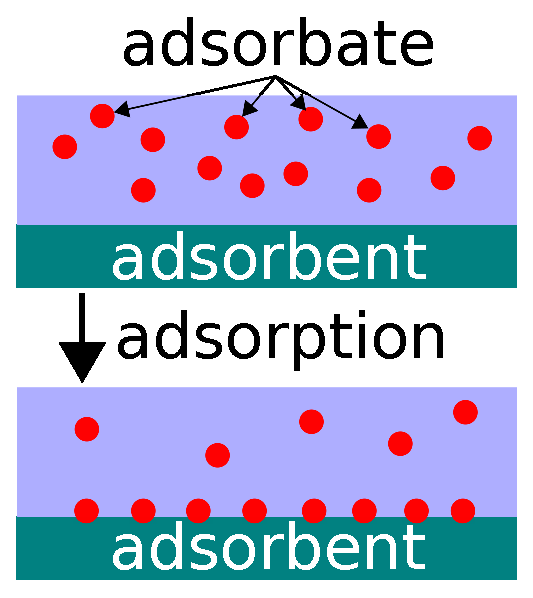
\includegraphics[width=0.25\textwidth]{adsorption.eps}
\caption{During adsorption, a thin adhered layer of the adsorbate is produced on the surface of the adsorbent.}
\label{fig:adsorption}
\end{SCfigure}
The original media from which the adsorbate originates can be gas or liquid.
The reverse process is called desorption.
Adsorption is an important process, and it is present in many areas of everyday life, industry, research, pharmacy.
It is an important step -- among many -- in heterogeneous catalysis, water treatment, removal by activated carbon.
Adsorption by activated carbon is used to remove toxins or unwanted dangerous substances from the gastrointestinal tract after poisonings.
Adsorption can be used in pharmaceutical industry to modulate the rate at which specific components are being released. 
It is the basis of many types of chromatography.

The first theoretical model to describe adsorption was developed by Irving Langmuir:

\begin{equation}
\label{eq:langmuir1}
        \theta
        =
        \frac
                {K p}
                {1 + K p} 
\end{equation}

It is called the \emph{Langmuir isotherm}, and its plot can be seen in Fig. \ref{fig:langmuir}. $\theta$ is the \emph{fractional coverage}, $K$ is $k_d/k_a$, the ratio of the rate of desorption and adsorption. $p$ is the partial pressure of the adsorbate.

\begin{figure}
\centering
\begin{tikzpicture}
\begin{axis}[xtick=\empty, xmin=0,xmax=10,ymin=0,ymax=1.1,xlabel={$c$}, ylabel={$\theta$},no markers,samples=50]
        \addplot[domain=0:10, black] {x/(x+1)};
        \draw [color=red, dashed] (0,100) -- (100,100);
        \draw [color=red, dashed] (10,0) -- (10,50);
	\draw [color=red, fill=red] (10,50) circle [radius=0.1cm];
	\draw [color=red, dashed] (0,50) -- (10,50);
\end{axis}
\end{tikzpicture}
\caption{The Langmuir isotherm. Red dot: $K$, the \emph{half-saturation constant}. $\theta$ eventually reaches 1 (maximal coverage), as $c$ approaches infinity. In practice, maximal coverage is reached much sooner.}
\label{fig:langmuir}
\end{figure}

This equation was derived to describe the adsorption of gases at solid surfaces. However, it also describes the adsorption of a solute from a solution, if the solvent has little or no adsorption to the adsorbent, compared to the solute. After replacing the partial pressure $p$ and multiplying both sides with the \emph{maximal adsorption capacity} $n_{max}$ we get:

\begin{equation}
\label{eq:langmuir2}
        n
        =
        n_{max}
	\frac
                {c}
                {c + K_{half}} 
\end{equation}

where $c$ is the equilibrium concentration of the adsorbate in the solution, $K_{half}$ is the \emph{half-saturation constant}, that equals to $1/K$. The half-saturation constant is the equilibrium concentration of the adsorbate, when half of the available surface is covered, so $\theta = 0.5$. Note that if $c = K_{half}$, then $c/(c + K_{half})$ is $1/2$ and therefore $n = 0.5\, n_{max}$. 

Specific adsorbance ($n^*_{max}$) is the amount of adsorbate adsorbed by 1 g of adsorbent. Its unit is mol/g. The maximal specific adsorption capacity of an adsorbent can be determined from the linearized form of Eq. \ref{eq:langmuir1}:

\begin{equation}
\label{eq:langmuir2}
        \frac{1}{n^*}
        =
        \frac{1}{n^*_{max}}
	+
	\frac{K'}{c}
\end{equation}

If we plot $1/n^*$ as a function of $1/c$, then the $y$-interception will be $1/n^*_{max}$. Determining it is the goal of the practice.

\subsection{Practice procedures}

Prepare a dilution series from known concentration methylene blue stock solution. The series should feature the following concentrations: $2\cdot10^{-4}$, $10^{-4}$, $5\cdot10^{-5}$, $2\cdot10^{-5}$, $10^{-5}$, $5\cdot10^{-6}$ M. Use 50 ml volumetric flasks to prepare the solutions. Record a spectrum of the $2\cdot10^{-5}$ solution, and determine the absorption peak in the visible range. Measure the absorbance of all the solutions. This dataset will be used to prepare the calibration curve.

Pipette 25--25 ml from each solution into a 100 ml Erlenmeyer flask. Put 0.3--0.5 g of adsorbent into each of flasks. The mass should be known in each case. The absorbent will be cellullose (filter paper or cotton swab) on the practice.
Shake the solutions for 30 minutes, then filter them, and measure their absorbance.

Calculate the adsorbed amount, and prepare the $1/n^*$--$1/c$ plot based on Eq. \ref{eq:langmuir2}. Correct for the differences in adsorbent mass by using the specific adsorbance.
After doing a linear regression (line fitting) on the dataset, use the $y$--interception to calculate $n^*_{max}$. 

%Written, updated and translated by András Kiss in 2017.

\newpage
\fancyhead[LE,RO]{Appendix A -- Ionic conductivity at infinite dilution}
\fancyhead[LO,RE]{\thesection}
\fancyfoot[LE,RO]{\thepage}
\fancyfoot[RE,LO]{\emph{Physical chemistry laboratory practice}}

\section*{Appendix A -- Ionic conductivity at infinite dilution}
\addcontentsline{toc}{section}{Appendix A -- Ionic conductivity at infinite dilution}
The following table includes the molar ionic conductivities at infinite dilution for certain ions, that are necessary for evaluations in certain practices. The values refer to aqueous solutions at 25 $\celsius$.

\begin{table}[h!]
\centering
\caption{Molar ionic conductivity at infinite dilution. Source: CRC Handbook of Chemistry and Physics 76th edition, David R. Lide editor in chief, 1995-1996 ISBN: 0-8493-0476-8.}
\label{table:conductivities}
\vspace{5mm}
\begin{tabular}{l|c}
%\hline
                        Ion \hspace{2cm} & $\lambda^0_\pm$, $\cdot$10$^{-4}\cdot$m$^2 \cdot$S$\cdot$mol$^{-1}$\\
                      \hline


Ag$^+$ \dotfill & 61.9 \\
1/3 Al$^{3+}$ \dotfill& 61 \\
1/2 Ba$^{2+}$\dotfill& 63.6 \\
1/2 Be$^{2+}$\dotfill& 45 \\
1/2 Ca$^{2+}$\dotfill& 59.47 \\
1/2 Cd$^{2+}$\dotfill& 54 \\
1/3 Ce$^{3+}$\dotfill& 69.8 \\
1/2 Co$^{2+}$\dotfill& 55 \\
%1/3 [Co(NH$_3$)$_6$]$^{3+}$\dotfill& \\
%1/3 [Co(en)$_3$]$^{3+}$\dotfill& \\
%1/6 [Co$_2$(trien)$_3$]$^{6+}$\dotfill& \\
%1/3 Cr$^{3+}$\dotfill& \\
%Cs$^+$\dotfill& \\
1/2 Cu$^{2+}$\dotfill& 69.3 \\
%D$^+$\dotfill& \\
%1/3 Dy$^{3+}$\dotfill& \\
%1/3 Er$^{3+}$\dotfill& \\
%1/3 Eu$^{3+}$\dotfill& \\
1/2 Fe$^{2+}$\dotfill& 54 \\
1/3 Fe$^{3+}$\dotfill& 68 \\
%1/3 Gd$^{3+}$\dotfill& \\
H$^+$\dotfill& 67.3 \\
1/2 Hg$^{2+}$\dotfill& 68.6 \\
%1/2 Hg$^{2+}$\dotfill& \\
%1/3 Ho$^{3+}$\dotfill& \\
K$^+$\dotfill& 73.48 \\
%1/3 La$^{3+}$\dotfill& \\
%Li$^+$\dotfill& \\
1/2 Mg$^{2+}$\dotfill& 53.0 \\
%1/2 Mn$^{2+}$\dotfill& \\
%NH$_4^{+}$\dotfill& \\
%N$_2$H$_5^+$\dotfill& \\
1/2 CO$_3^{2-}$\dotfill & 69.3 \\

\end{tabular}
\end{table}

%\newpage
%\fancyhead[LE,RO]{Investigating a ternary system -- ,,TER''}
\fancyhead[LO,RE]{\thesection}
\fancyfoot[LE,RO]{\thepage}
\fancyfoot[RE,LO]{\emph{Physical chemistry laboratory practice}}

\section{Investigating a ternary system}
\subsection{Introduction}

Ternary systems pose interesting questions not only form a theoretical point of view, but they also have practical importance for instance in metallurgy or the plastic industry. Just consider alloys, in which several different solid phases could be present, or mutually insoluble liquid phases which contain a common dissolved substance, for instance a drug dissolved in fat and water. In a ternary system, the mutual solubility of the components could be different. In every ternary system there is a pressure and/or temperature at which at least two components are only partially soluble in each other. The presence of a third component -- in case it mixes partially or completely in the other two -- could modifiy the mutual solubility of the two other components.

If the components are not reacting with each other, then to describe the state of a ternary system, knowing the temperature and the pressure is necessary. Since knowing the molefraction of two components determines the molefraction of third, the degree of freedom in such a system is 4. Therefore, at a given temperature and pressure, we only have to know the molefraction of two of the components to know the exact state of the system. To plot the phase diagramm of a ternary system on a plane, it is useful to take pressure and temperature constant. By doing this, the phase diagramm of the system can be plotted on an equilateral triangle. The corners of the triangle represent a system composed of only one of the three components. For easier reading, there is a convention regarding the orientation of the axes of the ternary triangle; it is always counter-clockwise. The sides (axes) of the triangle, the mole or weigth fraction or percentage of the components are represented (Fig. \ref{fig:1}.). Point \emph{,,P''} inside the triangle represents a system with all three components. We can read the composition by finding the respective molefraction values on the axes. The sides gives the composition of the pairwise two-component systems as well (Fig. \ref{fig:2} I.). In Fig. \ref{fig:2}. (I.) we show the composition of a ternary system, in which two components mix partially (water--chloroform), while the third (acetic acid for instance) dissolves completely in both. The area below the curve marks the heterogeneous systems. In such a state, the system will have two, so-called \emph{,,conjugated phases''}. Any point in the triangle outside of this area represents a homnogeneous system. Where the curve intersects any side of the triangle, the system has two components; x$_{A,1}$ and x$_{C,1}$ mean the solubility of water in chloroform, x$_{A,2}$ and x$_{C,2}$ mean the solubility of chloroform in water, if A is water, B is acetic acid and C is chloroform. If all the component pairs are only partially soluble in each other, then we get a diagramm similar to Fig. \ref{fig:2}. (II.).

From now on we discuss the water--chloroform--acetic acid ternary system. As we have mentioned already, any point below the curve will mean a system with two conjugated phases. Connecting the two points that are representing the conjugated phases we get the so called \emph{,,tie line''}. All the tie lines will have a common intersection, usually outside of the triangle (point \emph{P}, Fig. \ref{fig:3}). The tie lines are usually not parallel with the base of the triangle, because the third component doesn't dissolve equally in the two conjugated phases. Drawing a tangent from pont P to the curve we get point \emph{K}, the \emph{plait point} for a given temperature and pressure. If not all one but two or three component pairs are only partially miscible in each other, the we get two or three plait points, respectively. In the practice we will investigate the water-chloroform-acetic acid ternary system. 

\subsection{Practice procedures}

Prepare 20 cm$^3$ 15, 30, 50, 60, 70, 80, 85, 90 and 95 volume\% mixtures of chloroform and acetic acid. The volume\% is given with respect to chloroform. Measure the components with an automatic burette into clean, water-free Erlenmeyer flasks, and close them. Titrate the mixtures with water using a graduated (0.05 cm$^3$) 10 cm$^3$ automatic burette until you observe a slight opaque white color throughout the mixture. Find the density of the components from the table below, and using these and the volumes used until the endpoints (opaque color) calculate the mole fraction and mass fractoin of all three components for all 9 mixtures. Draw the two phase diagramms, using both mole and mass fraction as well (two separate diagramms) to get the equilibrium diagramm. Give the results of the calculations in a table such as the following:


To determine the plate point, prepare a mixture which has two conjugated phases (system under the curve). Separate them, and titrate a known mass of both of them with NaOH to get the mass of acetic acid in both of them. Then calculate the mass fraction of acetic acid in the conjugated phases. After this step we can draw a tie line. Repeat it with another mixture with different composition, to get an additional tie line. Draw a tangent from the intersection of the tie lines to get the plait point. Give the mass fraction composition of this point as a final result of the practice.

Recommandations for the two systems:

\begin{itemize}
\item A: 20 ml water, 25 ml chloroform, 1 ml acetic acid
\item B: 25 ml water, 25 ml chloroform, 3 ml acetic acid
\end{itemize}

Close the flasks, shake them for about 5 minutes to reach equilibrium. Separate the phases in a separation funnel, and titrate 5 ml of the organic and 10 ml of the water phase, after measuring the mass of both. Use either 0.1 M or 1 M NaOH fot titration and a few drops of phenolphthalein as indicator. Prepare the following table:


Knowing the mass of the phases you can calculate the mass fraction of acetic acid in both phases. Using these, find the intersection with the equlibrium line to get the conjugated phases' composition. Draw both tie lines. Find point P, the intersection of the tie lines. Draw the tangent to the equilibrium line from point P, to get the plait point K. Read the mass fraction composition of the plait point and write it down in your notebook as a final conclusion.  


\begin{figure}
\includegraphics{fig/ternary_diagram.pdf}
\end{figure}
%\begin{tikzpicture}
%\begin{ternaryaxis}[
%	%title=The water--chloroform--acetic acid ternary system,
%	xlabel=Weight percent of acetic acid,
%	ylabel=Weight percent of chloroform,
%	zlabel=Weight percent of water,
%	label style=sloped,
%	area style,
%]
%	\addplot3 table {
%	0 0.1 0.9
%	 
%	0.28 0.35 0.37
%	0.25 0.6 0.15
%	0.1 0.9 0
%	0 1 0
%	0 0 1
%	};
%	%\addlegendentry{$\gamma$FeNi}
%
%	%\node[inner sep=0.5pt,circle,draw,fill=white,pin=-15:\footnotesize Stainless Steel] at (axis cs:0.18,0.74,0.08) {};
%	
%\end{ternaryaxis}
%\end{tikzpicture}






\end{document}
